\documentclass[journal,12pt,twocolumn]{IEEEtran}
%
\usepackage{setspace}
\usepackage{gensymb}
\usepackage{xcolor}
\usepackage{caption}
%\usepackage{subcaption}
%\doublespacing
\singlespacing

%\usepackage{graphicx}
%\usepackage{amssymb}
%\usepackage{relsize}
\usepackage[cmex10]{amsmath}
\usepackage{mathtools}
%\usepackage{amsthm}
%\interdisplaylinepenalty=2500
%\savesymbol{iint}
%\usepackage{txfonts}
%\restoresymbol{TXF}{iint}
%\usepackage{wasysym}
\usepackage{hyperref}
\usepackage{amsthm}
\usepackage{mathrsfs}
\usepackage{txfonts}
\usepackage{stfloats}
\usepackage{cite}
\usepackage{cases}
\usepackage{subfig}
%\usepackage{xtab}
\usepackage{longtable}
\usepackage{multirow}
%\usepackage{algorithm}
%\usepackage{algpseudocode}
%\usepackage{enumerate}
\usepackage{enumitem}
\usepackage{mathtools}
%\usepackage{iithtlc}
%\usepackage[framemethod=tikz]{mdframed}
\usepackage{listings}


%\usepackage{stmaryrd}


%\usepackage{wasysym}
%\newcounter{MYtempeqncnt}
\DeclareMathOperator*{\Res}{Res}
%\renewcommand{\baselinestretch}{2}
\renewcommand\thesection{\arabic{section}}
\renewcommand\thesubsection{\thesection.\arabic{subsection}}
\renewcommand\thesubsubsection{\thesubsection.\arabic{subsubsection}}

\renewcommand\thesectiondis{\arabic{section}}
\renewcommand\thesubsectiondis{\thesectiondis.\arabic{subsection}}
\renewcommand\thesubsubsectiondis{\thesubsectiondis.\arabic{subsubsection}}

%\renewcommand{\labelenumi}{\textbf{\theenumi}}
%\renewcommand{\theenumi}{P.\arabic{enumi}}

% correct bad hyphenation here
\hyphenation{op-tical net-works semi-conduc-tor}

\lstset{
language=Python,
frame=single, 
breaklines=true,
columns=fullflexible
}



\begin{document}
%

\theoremstyle{definition}
\newtheorem{theorem}{Theorem}[section]
\newtheorem{problem}{Problem}
\newtheorem{proposition}{Proposition}[section]
\newtheorem{lemma}{Lemma}[section]
\newtheorem{corollary}[theorem]{Corollary}
\newtheorem{example}{Example}[section]
\newtheorem{definition}{Definition}[section]
%\newtheorem{algorithm}{Algorithm}[section]
%\newtheorem{cor}{Corollary}
\newcommand{\BEQA}{\begin{eqnarray}}
\newcommand{\EEQA}{\end{eqnarray}}
\newcommand{\define}{\stackrel{\triangle}{=}}
\newcommand{\myvec}[1]{\ensuremath{\begin{pmatrix}#1\end{pmatrix}}}
\bibliographystyle{IEEEtran}
%\bibliographystyle{ieeetr}

\providecommand{\nCr}[2]{\,^{#1}C_{#2}} % nCr
\providecommand{\nPr}[2]{\,^{#1}P_{#2}} % nPr
\providecommand{\mbf}{\mathbf}
\providecommand{\pr}[1]{\ensuremath{\Pr\left(#1\right)}}
\providecommand{\qfunc}[1]{\ensuremath{Q\left(#1\right)}}
\providecommand{\sbrak}[1]{\ensuremath{{}\left[#1\right]}}
\providecommand{\lsbrak}[1]{\ensuremath{{}\left[#1\right.}}
\providecommand{\rsbrak}[1]{\ensuremath{{}\left.#1\right]}}
\providecommand{\brak}[1]{\ensuremath{\left(#1\right)}}
\providecommand{\lbrak}[1]{\ensuremath{\left(#1\right.}}
\providecommand{\rbrak}[1]{\ensuremath{\left.#1\right)}}
\providecommand{\cbrak}[1]{\ensuremath{\left\{#1\right\}}}
\providecommand{\lcbrak}[1]{\ensuremath{\left\{#1\right.}}
\providecommand{\rcbrak}[1]{\ensuremath{\left.#1\right\}}}
\theoremstyle{remark}
\newtheorem{rem}{Remark}
\newcommand{\sgn}{\mathop{\mathrm{sgn}}}
\providecommand{\abs}[1]{\left\vert#1\right\vert}
\providecommand{\res}[1]{\Res\displaylimits_{#1}} 
\providecommand{\norm}[1]{\lVert#1\rVert}
\providecommand{\mtx}[1]{\mathbf{#1}}
\providecommand{\mean}[1]{E\left[ #1 \right]}
\providecommand{\fourier}{\overset{\mathcal{F}}{ \rightleftharpoons}}
\providecommand{\ztrans}{\overset{\mathcal{Z}}{ \rightleftharpoons}}

%\providecommand{\hilbert}{\overset{\mathcal{H}}{ \rightleftharpoons}}
\providecommand{\system}{\overset{\mathcal{H}}{ \longleftrightarrow}}
	%\newcommand{\solution}[2]{\textbf{Solution:}{#1}}
\newcommand{\solution}{\noindent \textbf{Solution: }}
\providecommand{\dec}[2]{\ensuremath{\overset{#1}{\underset{#2}{\gtrless}}}}
\numberwithin{equation}{section}
%\numberwithin{equation}{subsection}
%\numberwithin{problem}{subsection}
%\numberwithin{definition}{subsection}
\makeatletter
\@addtoreset{figure}{problem}
\makeatother

\let\StandardTheFigure\thefigure
%\renewcommand{\thefigure}{\theproblem.\arabic{figure}}
\renewcommand{\thefigure}{\theproblem}


%\numberwithin{figure}{subsection}

\def\putbox#1#2#3{\makebox[0in][l]{\makebox[#1][l]{}\raisebox{\baselineskip}[0in][0in]{\raisebox{#2}[0in][0in]{#3}}}}
     \def\rightbox#1{\makebox[0in][r]{#1}}
     \def\centbox#1{\makebox[0in]{#1}}
     \def\topbox#1{\raisebox{-\baselineskip}[0in][0in]{#1}}
     \def\midbox#1{\raisebox{-0.5\baselineskip}[0in][0in]{#1}}

\vspace{3cm}

\title{ 
%\logo{
Digital Signal Processing
%}
%	\logo{Octave for Math Computing }
}
%\title{
%	\logo{Matrix Analysis through Octave}{\begin{center}\includegraphics[scale=.24]{tlc}\end{center}}{}{HAMDSP}
%}


% paper title
% can use linebreaks \\ within to get better formatting as desired
%\title{Matrix Analysis through Octave}
%
%
% author names and IEEE memberships
% note positions of commas and nonbreaking spaces ( ~ ) LaTeX will not break
% a structure at a ~ so this keeps an author's name from being broken across
% two lines.
% use \thanks{} to gain access to the first footnote area
% a separate \thanks must be used for each paragraph as LaTeX2e's \thanks
% was not built to handle multiple paragraphs
%

\author{I Sai Pradeep% <-this % stops a space
%\thanks{J. Doe and J. Doe are with Anonymous University.}% <-this % stops a space
%\thanks{Manuscript received April 19, 2005; revised January 11, 2007.}}
}
% note the % following the last \IEEEmembership and also \thanks - 
% these prevent an unwanted space from occurring between the last author name
% and the end of the author line. i.e., if you had this:
% 
% \author{....lastname \thanks{...} \thanks{...} }
%                     ^------------^------------^----Do not want these spaces!
%
% a space would be appended to the last name and could cause every name on that
% line to be shifted left slightly. This is one of those "LaTeX things". For
% instance, "\textbf{A} \textbf{B}" will typeset as "A B" not "AB". To get
% "AB" then you have to do: "\textbf{A}\textbf{B}"
% \thanks is no different in this regard, so shield the last } of each \thanks
% that ends a line with a % and do not let a space in before the next \thanks.
% Spaces after \IEEEmembership other than the last one are OK (and needed) as
% you are supposed to have spaces between the names. For what it is worth,
% this is a minor point as most people would not even notice if the said evil
% space somehow managed to creep in.



% The paper headers
%\markboth{Journal of \LaTeX\ Class Files,~Vol.~6, No.~1, January~2007}%
%{Shell \MakeLowercase{\textit{et al.}}: Bare Demo of IEEEtran.cls for Journals}
% The only time the second header will appear is for the odd numbered pages
% after the title page when using the twoside option.
% 
% *** Note that you probably will NOT want to include the author's ***
% *** name in the headers of peer review papers.                   ***
% You can use \ifCLASSOPTIONpeerreview for conditional compilation here if
% you desire.




% If you want to put a publisher's ID mark on the page you can do it like
% this:
%\IEEEpubid{0000--0000/00\$00.00~\copyright~2007 IEEE}
% Remember, if you use this you must call \IEEEpubidadjcol in the second
% column for its text to clear the IEEEpubid mark.



% make the title area
\maketitle

%\newpage

\tableofcontents

%\renewcommand{\thefigure}{\thesection.\theenumi}
%\renewcommand{\thetable}{\thesection.\theenumi}

\renewcommand{\thefigure}{\theenumi}
\renewcommand{\thetable}{\theenumi}

%\renewcommand{\theequation}{\thesection}



\bigskip

\begin{abstract}
This manual provides a simple introduction to digital signal processing.
\end{abstract}
\section{Software Installation}
Run the following commands
\begin{lstlisting}
sudo apt-get update
sudo apt-get install libffi-dev libsndfile1 python3-scipy  python3-numpy python3-matplotlib 
sudo pip install cffi pysoundfile 
\end{lstlisting}
\section{Digital Filter}
\begin{enumerate}[label=\thesection.\arabic*
,ref=\thesection.\theenumi]
\item
\label{prob:input}
Download the sound file from  
\begin{lstlisting}
wget https://github.com/AvinashNayak27/digital/blob/master/codes/Sound_Noise.wav
\end{lstlisting}
%\href{http://tlc.iith.ac.in/img/sound/Sound_Noise.wav}{\url{http://tlc.iith.ac.in/img/sound/Sound_Noise.wav}}  
%in the link given below.
%\linebreak
\item
\label{prob:spectrogram}
You will find a spectrogram at \href{https://academo.org/demos/spectrum-analyzer}{\url{https://academo.org/demos/spectrum-analyzer}}. 
%\end{problem}
%%
%
%%\onecolumn
%%\input{./figs/fir}
%\begin{problem}
Upload the sound file that you downloaded in Problem \ref{prob:input} in the spectrogram  and play.  Observe the spectrogram. What do you find?
\\
%
\solution There are a lot of yellow lines between 440 Hz to 5.1 KHz.  These represent the synthesizer key tones. Also, the key strokes
are audible along with background noise.
% By observing spectrogram, it clearly shows that tonal frequency is under 4kHz. And above 4kHz only noise is present.
\item
\label{prob:output}
Write the python code for removal of out of band noise and execute the code.
\\
\solution
\lstinputlisting{./codes/Cancel_noise.py}
%\begin{figure}[h]
%\centering
%\includegraphics[width=\columnwidth]{enc_block_diag.png}
%\caption{}
%\label{fig:convolution encoder}
%\end{figure}
%\input{block_enc}
\item
The output of the python script in Problem \ref{prob:output} is the audio file Sound\_With\_ReducedNoise.wav. Play the file in the spectrogram in Problem \ref{prob:spectrogram}. What do you observe?
\\
\solution The key strokes as well as background noise is subdued in the audio.  Also,  the signal is blank for frequencies above 5.1 kHz.

\end{enumerate}
\section{Difference Equation}
\begin{enumerate}[label=\thesection.\arabic*,ref=\thesection.\theenumi]
\item Let
	\label{def:xn}
\begin{equation}
x(n) = \cbrak{\underset{\uparrow}{1},2,3,4,2,1}
\end{equation}
Sketch $x(n)$.
\item Let
\begin{multline}
\label{eq:iir_filter}
y(n) + \frac{1}{2}y(n-1) = x(n) + x(n-2), 
\\
 y(n) = 0, n < 0
\end{multline}
Sketch $y(n)$.  
\\
\solution The following code yields Fig. \ref{fig:xnyn}.
\begin{lstlisting}
wget https://github.com/AvinashNayak27/digital/blob/master/codes/xnyn.py
\end{lstlisting}
\begin{figure}[!ht]
\begin{center}
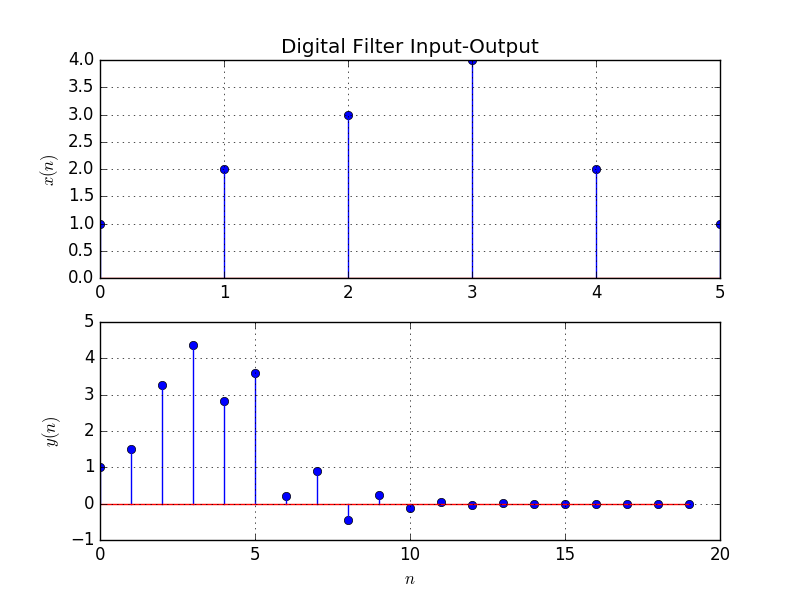
\includegraphics[width=\columnwidth]{./figs/xnyn}
\end{center}
\captionof{figure}{}
\label{fig:xnyn}	
\end{figure}
\item Repeat the above exercise using a C code.\\
 \solution Download the C code from the below link,
   \begin{lstlisting}
wget https://github.com/AvinashNayak27/digital/blob/master/codes/3.3.1.c
   \end{lstlisting}
   Then run the follwing command in terminal
    \begin{lstlisting}
gcc 3.3.1.c
./a.out
    \end{lstlisting}
    Then for the plot $\ref{3.3}$ download the python file from the below link,
    \begin{lstlisting}
wget https://github.com/AvinashNayak27/digital/blob/master/codes/3.3.2.py
    \end{lstlisting}
    Then run the command
    \begin{lstlisting}
python3 3.3.2.py
    \end{lstlisting}
    \begin{figure}[ht!]
      \centering
      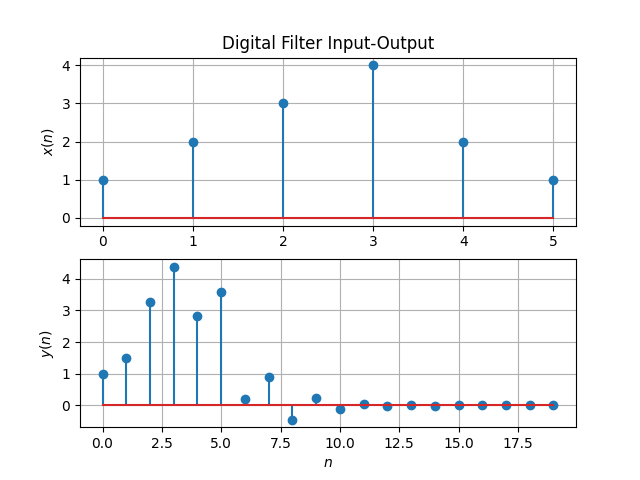
\includegraphics[width= \columnwidth]{figs/3.3.png}
      \caption{Plot using C code}
      \label{xnyn2}
    \end{figure}

\end{enumerate}
\section{$Z$-transform}
\begin{enumerate}[label=\thesection.\arabic*]
\item The $Z$-transform of $x(n)$ is defined as 
%
\begin{equation}
\label{eq:z_trans}
X(z)={\mathcal {Z}}\{x(n)\}=\sum _{n=-\infty }^{\infty }x(n)z^{-n}
\end{equation}
%
Show that
\begin{equation}
\label{eq:shift1}
{\mathcal {Z}}\{x(n-1)\} = z^{-1}X(z)
\end{equation}
and find
\begin{equation}
	{\mathcal {Z}}\{x(n-k)\} 
\end{equation}
\solution Given that,
  \begin{align}
     X\brak{z} &= \mathcal{Z}\cbrak{x\brak{n}}\\
               &= \sum_{n = -\infty}^{\infty}x\brak{n}z^{-n}
  \end{align}
  So,
   \begin{align}
     \mathcal{Z}\cbrak{x\brak{n-1}} &= \sum_{n=-\infty}^{\infty}x\brak{n-1}z^{-n}
   \end{align}
   Take $k = n-1$,
   \begin{align}
           &= \sum_{k=-\infty}^{\infty}x\brak{k}z^{-\brak{k+1}}\\
           &= z^{-1}\sum_{k=-\infty}^{\infty}x\brak{k}z^{-k}\\
           &= z^{-1}\sum_{n=-\infty}^{\infty}x\brak{n}z^{-n}\\
           &= z^{-1}X\brak{z}    
   \end{align}
   resulting in $\eqref{eq:shift1}$ and similarly following the above steps you will get,
     \begin{align}
          \mathcal{Z}\cbrak{x\brak{n-k}} &= z^{-k}X\brak{n}\label{shift_k_Z_transform}
     \end{align} 
   Hence proved.
    \item Obtain $X(z)$ for $x(n)$ defined in problem 
    \ref{def:xn}.
    \solution 
    Now we will find $Z$ transform of the signal $x\brak{n}$,from $\eqref{xn}$,
    \begin{align}
      \mathcal{Z}\cbrak{x\brak{n}} &= \sum_{n=0}^{5}x\brak{n}z^{-n}\\
                                   &= 1z^{0} + 2z^{-1} + 3z^{-2}+4z^{-3} + 2z^{-4} +1z^{-5}\\
                                   &= 1 + 2z^{-1} + 3z^{-2} + 4z^{-3} + 2z^{-4} + z^{-5} 
    \end{align}
   \item Find
   %
   \begin{equation}
   H(z) = \frac{Y(z)}{X(z)}
   \end{equation}
   %
   from  $\eqref{eq:iir_filter}$ assuming that the $Z$-transform is a linear operation.
   \\
   \solution Applying \eqref{shift_k_Z_transform} in \eqref{eq:iir_filter},
   \begin{align}
   Y(z) + \frac{1}{2}z^{-1}Y(z) &= X(z)+z^{-2}X(z)
   \\
   \implies \frac{Y(z)}{X(z)} &= \frac{1 + z^{-2}}{1 + \frac{1}{2}z^{-1}}
   \label{eq:freq_resp}
   \end{align}
   %
    \solution 
     Now we will rewrite $\eqref{eq:iir_filter}$,
      \begin{align}
          y(n) + \frac{1}{2}y(n-1) = x(n) + x(n-2)
      \end{align}
     Now since $Z$-transform is a linear operator we can write that,
      \begin{align}
          Y\brak{n} + \frac{1}{2}Y\brak{n-1} &= X\brak{n} + X\brak{n-2}
      \end{align}
      From $\eqref{shift_k_Z_transform}$,
      \begin{align}
          Y\brak{n} + \frac{z^{-1}}{2}Y\brak{n} &= X\brak{n} + z^{-2}X\brak{n}\\
       \implies \frac{Y\brak{n}}{X\brak{n}} &= \frac{1 + z^{-2}}{1 + \frac{z^{-1}}{2}} 
      \end{align}       
      \item Find the Z transform of 
      \begin{equation}
      \label{delta}
      \delta(n)
      =
      \begin{cases}
      1 & n = 0
      \\
      0 & \text{otherwise}
      \end{cases}
      \end{equation}
      and show that the $Z$-transform of
      \begin{equation}
      \label{eq:unit_step}
      u(n)
      =
      \begin{cases}
      1 & n \ge 0
      \\
      0 & \text{otherwise}
      \end{cases}
      \end{equation}
      is
      \begin{equation}
      U(z) = \frac{1}{1-z^{-1}}, \quad \abs{z} > 1
      \end{equation}
      \solution 
      The $Z$-transform of $\delta{n}$ is,
      \begin{align}
          \mathcal{Z}\cbrak{\delta{n}} &= \sum_{n=-\infty}^{\infty}\delta\brak{n}z^{-n}\\
                                       &= \delta\brak{0}z^{0} + 0\,\, \brak{\text{Using \eqref{delta}}}\\
                                       &= 1
      \end{align}
       and the $Z$-transform of unit-step function $u\brak{n}$ is,
      \begin{align}
          U\brak{n} &= \sum_{n=-\infty}^{\infty}u\brak{n}z^{-n}\\
                    &= 0 + \sum_{n = 0}^{\infty}1.z^{-n}\\
                    &= 1 + z^{-1} + z^{-2} + .\,.\,.
      \end{align}
       Above is a infinite geometric series with $z^{-1}$ as common ratio , so we can write it as 
      \begin{align}
          U\brak{n} &= \frac{1}{1-z^{-1}} \because \abs{z} > 1
      \end{align} 
    \item Show that 
      \begin{equation}
        \label{eq:anun}
        a^nu(n) \ztrans \frac{1}{1-az^{-1}} \quad \abs{z} > \abs{a}
      \end{equation}
    \solution
     The $Z$- transform will be 
      \begin{align}
              \mathcal{Z}\cbrak{a^nu\brak{n}} &= \sum_{n = 0}^{\infty}a^{n}z^{-n}\\
                                              &= 1 + \frac{a}{z} + \brak{\frac{a}{z}}^2 + .\,.\,.\,.
      \end{align}
     Above is a infinite geometric series with first term $1$ and common ratio as $\frac{a}{z}$ and it can 
       be written as,
      \begin{align}
              \mathcal{Z}\cbrak{a^nu\brak{n}} &= \frac{1}{1 - \frac{a}{z}} \because \abs{a} < \abs{z} 
      \end{align}
     Therefore,
      \begin{equation}
          a^nu(n) \ztrans \frac{1}{1-az^{-1}} \quad \abs{z} > \abs{a}
      \end{equation}
    \item 
      Let
      \begin{equation}
        H\brak{e^{j \omega}} = H\brak{z = e^{j \omega}}.
      \end{equation}
      Plot $\abs{H\brak{e^{j \omega}}}$.  Comment.  $H(e^{j \omega})$ is known as the {\em Discret Time Fourier Transform} (DTFT) of $h(n)$.\\
    \solution
        Download the code for the plot $\ref{DTFT}$ from the link below
      \begin{lstlisting}
wget https://github.com/AvinashNayak27/digital/blob/master/codes/dtft.py
      \end{lstlisting}
      \begin{figure}[ht!]
        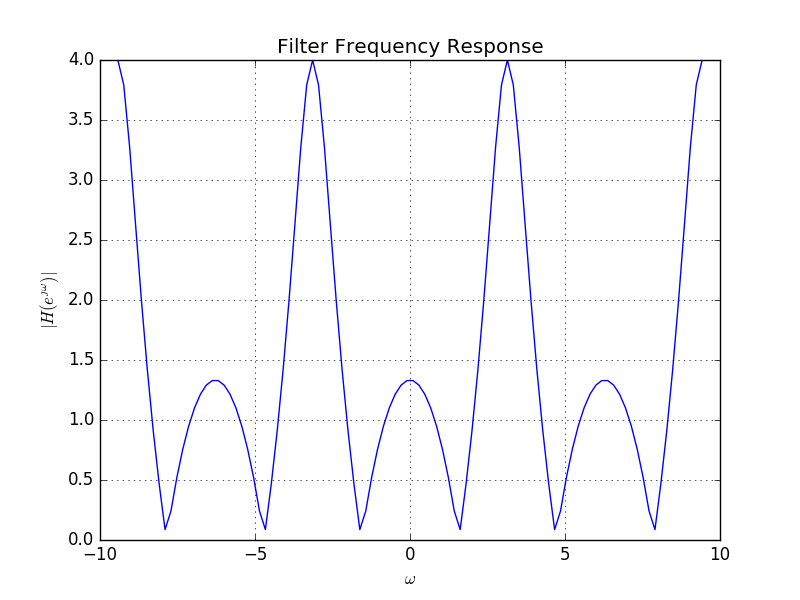
\includegraphics[width = \columnwidth]{Figs/dtft.png}
        \caption{$\abs{H\brak{e^{\j\omega}}}$}
        \label{DTFT}
      \end{figure} 
    Now using $\eqref{eq:freq_resp}$, we will find $\abs{H\brak{e^{j \omega}}}$,
     \begin{align}
      H\brak{e^{j \omega}} &= \frac{1+e^{-2j\omega}}{1 + \frac{e^{-j\omega}}{2}}\\
        \implies \abs{H\brak{e^{j \omega}}} &= \frac{\abs{1+e^{-2j\omega}}}{\abs{1 + \frac{e^{-j\omega}}{2}}}\\
                            &= \frac{\abs{1+e^{2j\omega}}}{\abs{e^{2j\omega} + \frac{e^{j\omega}}{2}}}\\
                            &= \frac{\abs{1+\cos2\omega + j\sin2\omega}}{\abs{e^{j\omega}+ \frac{1}{2}}}\\
                            &= \frac{\abs{4\cos^2\brak{\omega} + 4j\sin\brak{\omega}\cos\brak{\omega}}}{\abs{2e^{j\omega} + 1}}\\
                            &= \frac{\abs{4\cos\brak{\omega}}\abs{\cos\brak{\omega} + j\sin\brak{\omega}}}{\abs{2\cos\brak{\omega} + 1 + 2j\sin\brak{\omega}}}\\
        \therefore \abs{H\brak{e^{j \omega}}} &= \frac{\abs{4\cos\brak{\omega}}}{\sqrt{5 +4\cos\brak{\omega}}}
     \end{align}
Since $\abs{H(e^{j\omega})}$ is function of cosine we can say it is periodic.And from the plot $\ref{DTFT}$ we can say that it is symmetric about $\omega = 0\brak{\text{even function}}$ and it is periodic with period $2\pi$.You can find the same from the theoritical expression $\abs{H\brak{e^{j \omega}}}$, 
       \begin{align}
         H(e^{j\omega}) &= H(e^{j(-\omega)})\brak{\text{cos is an even function}}
       \end{align}
    And to find period, the period of $\abs{\cos(\omega)}$ is $\pi$ and the period of $\sqrt{5 + 4\cos\brak{\omega}}$ is $2\pi$. So the period of division of both will be,
     \begin{align}
      lcm\brak{\pi,2\pi} &= 2\pi
     \end{align}
     This gives us the period of $\abs{H(e^{j\omega})}$ as $2\pi$
  \item Express $h(n)$ in terms of $H\brak{e^{j \omega}}$.\\
  \solution We know that 
\begin{align}
	H(e^{j\omega})=\sum_{k=-\infty}^\infty h(k)e^{-j\omega k}
\end{align}



\begin{align}
  \implies
\frac{1}{2\pi}\int_{-\pi}^\pi& H(e^{j\omega})e^{j\omega n}d\omega\\
 &=\frac{1}{2\pi}\int_{-\pi}^\pi \sum_{k=-\infty}^\infty h(k)e^{-j\omega k}e^{j\omega n}d\omega\\
 &=\frac{1}{2\pi} \sum_{k=-\infty}^\infty h(k)\int_{-\pi}^\pi e^{j\omega (n-k)}d\omega\\
 &=\frac{1}{2\pi}\cbrak{ \sum_{k\neq n} h(k)\frac{e^{j\omega (n-k)}}{j(n-k)}\Biggr] _{-\pi}^\pi+h(n).{2\pi} }\\
 &=\frac{0+2\pi h(n)}{2\pi}\\
 &=h(n)
\end{align}
\begin{align}
	\therefore h(n)=\frac{1}{2\pi}\int_{-\pi}^\pi H(e^{j\omega})e^{j\omega n}d\omega 
\end{align}
    \end{enumerate}
    \section{Impulse Response}
    \begin{enumerate}[label=\thesection.\arabic*]
      \item Using long division, 
      find
      \begin{align}
        h(n), \quad n < 5
      \end{align}
      for H(z) in 
      \eqref{eq:freq_resp}.\\
      \solution $H(z)$ is given by
      \begin{align}
        H(z)=\frac{1+z^{-2}}{1+\frac{1}{2}z^{-1}}=\frac{2+2z^{-2}}{2+z^{-1}}
      \end{align}
      \begin{align}
        &2z^{-1}-4\\	
        z^{-1}+2\hspace{2mm}&\overline{\big)\hspace{2mm} 2z^{-2}+2\hspace{15mm}}\\
        & \hspace{2mm} 2z^{-2}+4z^{-1}\\
        &\overline{\hspace{11mm}-4z^{-1}+2\hspace{5mm}}\\
        &\hspace{9mm}-4z^{-1}-8\\ 
        &\overline{\hspace{24mm}10}
      \end{align}
      So,
      \begin{align}
        H(z)&=2z^{-1}-4+\frac{10}{z^{-1}+2}\\
        &=2z^{-1}-4+\frac{5}{\frac{1}{2}z^{-1}+1}\\
        &=2z^{-1}-4+5\sum_{n=0}^\infty \brak{-\frac{z^{-1}}{2}}^{n}\\
        &=1-\frac{1}{2}z^{-1}+\sum_{n=2}^\infty \brak{-\frac{1}{2}}^{n}z^{-n}
      \end{align}
      So,h(n) will be given by 
      \begin{align}
        h(n)=\begin{cases}
          \label{eq:h_n_def}
          5\times \brak{-\frac{1}{2}}^n  & n\geq 2\\
          \brak{-\frac{1}{2}}^n  &2>n\geq0\\
          0 &n<0
        \end{cases}
      \end{align}
      \item \label{prob:impulse_resp}
      Find an expression for $h(n)$ using $H(z)$, given that 
      %in Problem \ref{eq:ztransab} and \eqref{eq:anun}, given that
      \begin{equation}
        \label{eq:impulse_resp}
        h(n) \ztrans H(z)
      \end{equation}
      and there is a one to one relationship between $h(n)$ and $H(z)$. $h(n)$ is known as the {\em impulse response} of the
      system defined by \eqref{eq:iir_filter}.
      \\
      \solution From \eqref{eq:freq_resp},
      \begin{align}
        H(z) &= \frac{1}{1 + \frac{1}{2}z^{-1}} + \frac{ z^{-2}}{1 + \frac{1}{2}z^{-1}}
        \\
        \implies h(n) &= \brak{-\frac{1}{2}}^{n}u(n) + \brak{-\frac{1}{2}}^{n-2}u(n-2)
      \end{align}
      using \eqref{eq:anun} and \eqref{eq:z_trans_shift}.
      \item Sketch $h(n)$. Is it bounded? Justify theoreti-
      cally.
      \\
      \solution The following code plots Fig. \ref{fig:5.3}.
      \begin{lstlisting}
    wget https://github.com/Pradeep8802/EE3900-Digital-Signal-Processing/blob/main/Assignment1/codes/5.3.py
      \end{lstlisting}
      on simplfying we get h(n) as
      \begin{align}
        \begin{cases}
          %\label{eq:h_n_def}
          5\times \brak{-\frac{1}{2}}^n  & n\geq 2\\
          \brak{-\frac{1}{2}}^n  &2>n\geq0\\
          0 &n<0
        \end{cases}
      \end{align}
      \begin{align}
        \because 5\times \brak{-\frac{1}{2}}^n \to 0 \quad	\text{for} \quad n\to \infty 
      \end{align}
      So, we can conclude that h(n) is bounded.
      \begin{figure}[!ht]
        \centering
        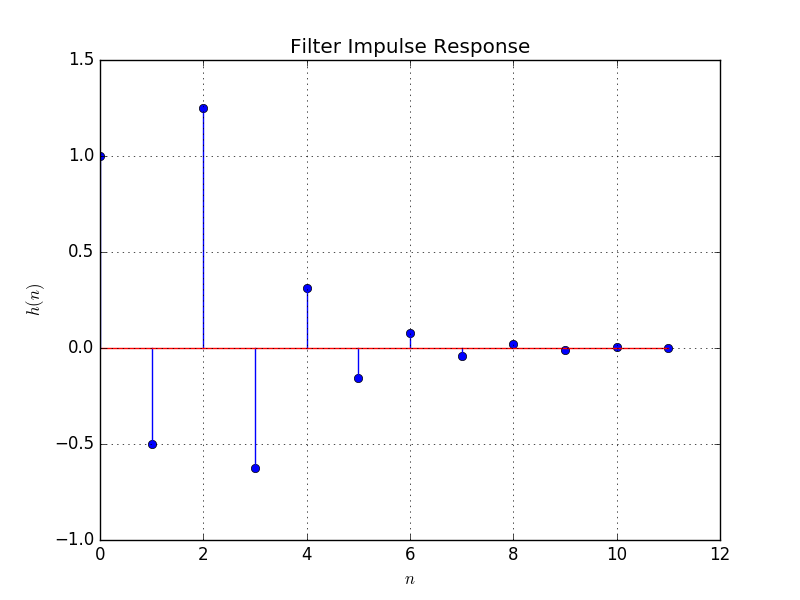
\includegraphics[width=\columnwidth]{./figs/hn.png}
        \caption{$h(n)$ wrt n}
        \label{fig:5.3}
      \end{figure}
      %
         \item Convergent? Justify using the ratio test.\\
    \solution We can say a given real sequence $\cbrak{x_n}$ is convergent if 
    \begin{align}
      \lim_{n \rightarrow \infty}\abs{\frac{x_{n+1}}{x_n}} < 1
    \end{align}
    This is known as Ratio test.\\
    In this case the limit will become,
    \begin{align}
      \lim_{n \rightarrow \infty}\abs{\frac{h\brak{n+1}}{h\brak{n}}} &= \lim_{n \rightarrow \infty}\abs{\frac{5\brak{\frac{-1}{2}}^{n+1}}{5\brak{\frac{-1}{2}}^{n}}} \\
      &= \lim_{n \rightarrow \infty}\abs{\frac{-1}{2}}\\
      &= \frac{1}{2}
    \end{align}
    As $\frac{1}{2} < 1$, from root test we can say that $h\brak{n}$ is convergent.
      \item The system with $h(n)$ is defined to be stable if
      \begin{equation}
        \sum_{n=-\infty}^{\infty}h(n) < \infty
      \end{equation}
      Is the system defined by \eqref{eq:iir_filter} stable for the impulse response in \eqref{eq:impulse_resp}?\\
      \solution For system of 3.2 ,$h(n)$ is defined in \eqref{eq:h_n_def} 
      So,
      \begin{align}
        \sum_{n=-\infty}^{\infty}h(n)&=\sum_{n=2}^{\infty}5\times \brak{-\frac{1}{2}}^n+\sum_{n=0}^{1} \brak{-\frac{1}{2}}^n+\sum_{n=-\infty}^{-1}0\\
        &=5\times \frac{1}{6}+\frac{1}{2}\\
        &=\frac{4}{3}
      \end{align}
      Since the sum is finite so the system is stable for impulsive response
      \item Verify the above result using a python code.\\
      \solution The above result is verified using the below python code
        \begin{lstlisting}
    wget https://github.com/Pradeep8802/EE3900-Digital-Signal-Processing/tree/main/Assignment1/codes/5.6.py
      \end{lstlisting}
      \item 
      Compute and sketch $h(n)$ using 
      \begin{equation}
        \label{eq:iir_filter_h}
        h(n) + \frac{1}{2}h(n-1) = \delta(n) + \delta(n-2), 
      \end{equation}
      %
      This is the definition of $h(n)$.
      \\
      \solution The following code plots Fig. \ref{fig:h_n_delta}. Note that this is the same as Fig. 
      \ref{fig:3.1}. 
      %
      \begin{lstlisting}
    wget https://github.com/Pradeep8802/EE3900-Digital-Signal-Processing/tree/main/Assignment1/codes/5.7.py
      \end{lstlisting}
      \begin{figure}[!ht]
        \centering
        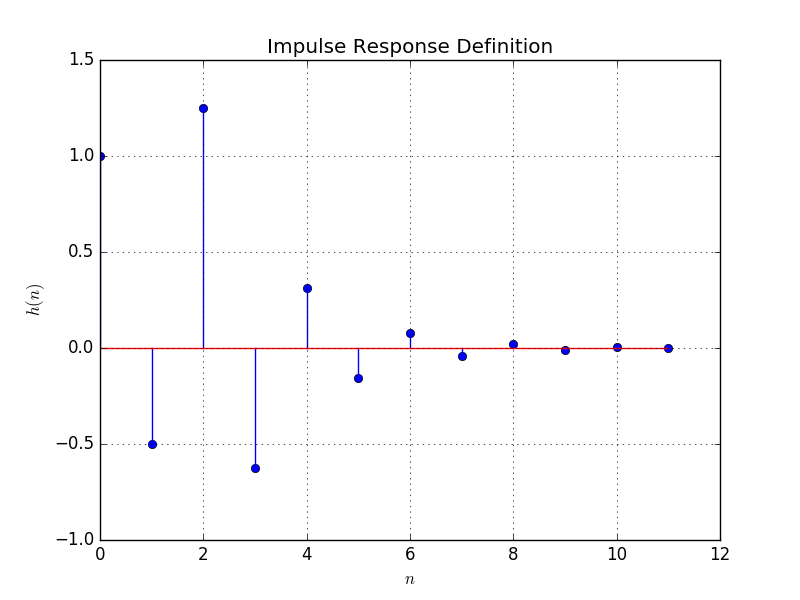
\includegraphics[width=\columnwidth]{figs/hndef.png}
        \caption{$h(n)$ from the definition}
        \label{fig:h_n_delta}
      \end{figure}
      %
      \item Compute 
      %
      \begin{equation}
        \label{eq:convolution}
        y(n) = x(n)*h(n) = \sum_{k=-\infty}^{\infty}x(k)h(n-k)
      \end{equation}
      %
      Comment. The operation in \eqref{eq:convolution} is known as
      {\em convolution}.
      %
      \\
      \solution The following code plots Fig. \ref{fig:y_n_convo}. Note that this is the same as 
      $y(n)$ in  Fig. 
      \ref{fig:3.1}. 
      \begin{lstlisting}
    wget https://github.com/Pradeep8802/EE3900-Digital-Signal-Processing/tree/main/Assignment1/codes/5.4.py
      \end{lstlisting}
      \begin{figure}[!ht]
        \centering
        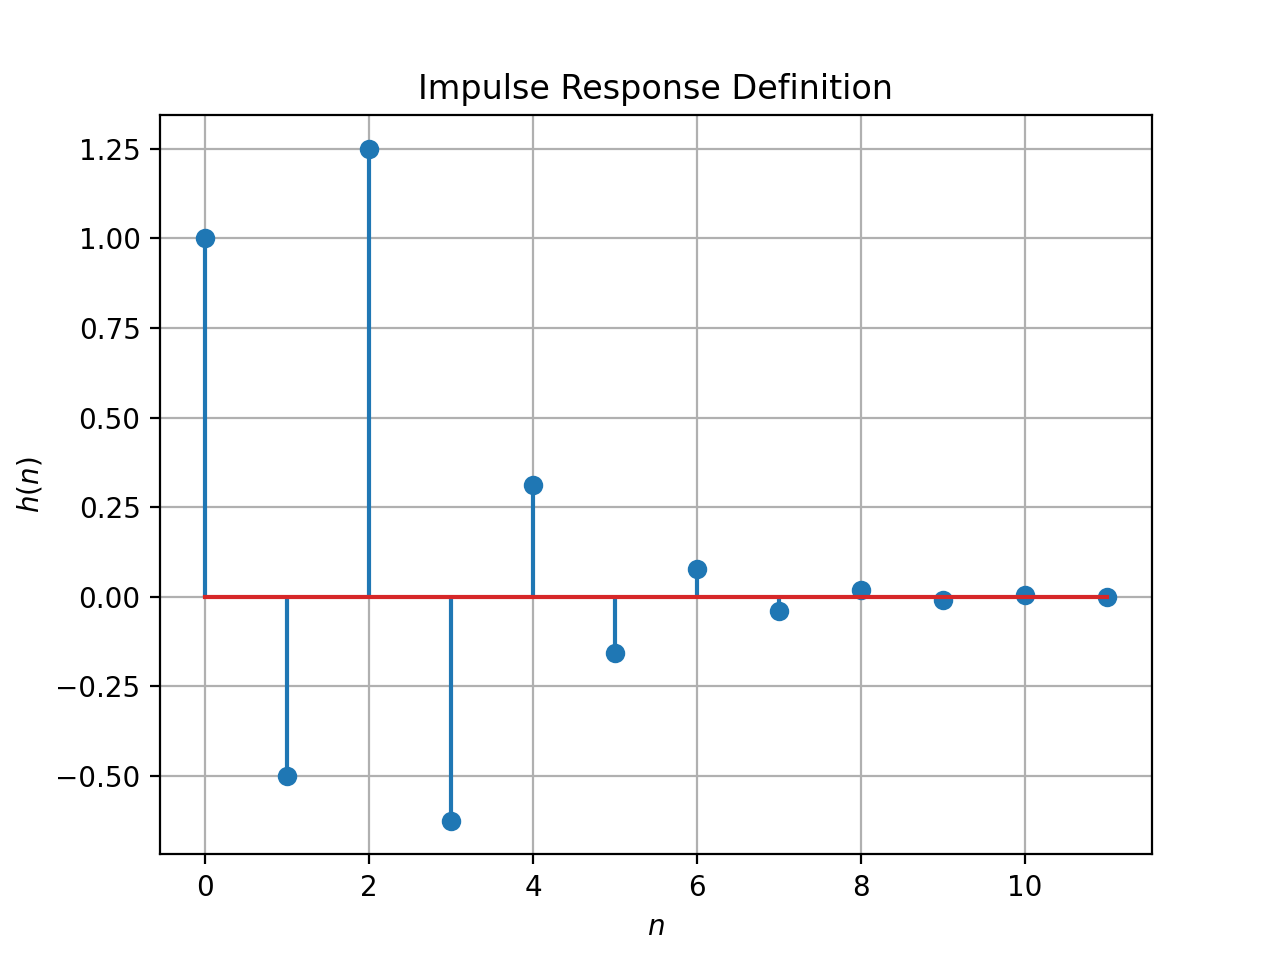
\includegraphics[width=\columnwidth]{figs/yndef.png}
        \caption{$y(n)$ from the definition of convolution}
        \label{fig:y_n_convo}
      \end{figure}
        \item Express the above convolution using a Toeplitz matrix.\\
      \solution 
      \begin{figure}
        \centering
        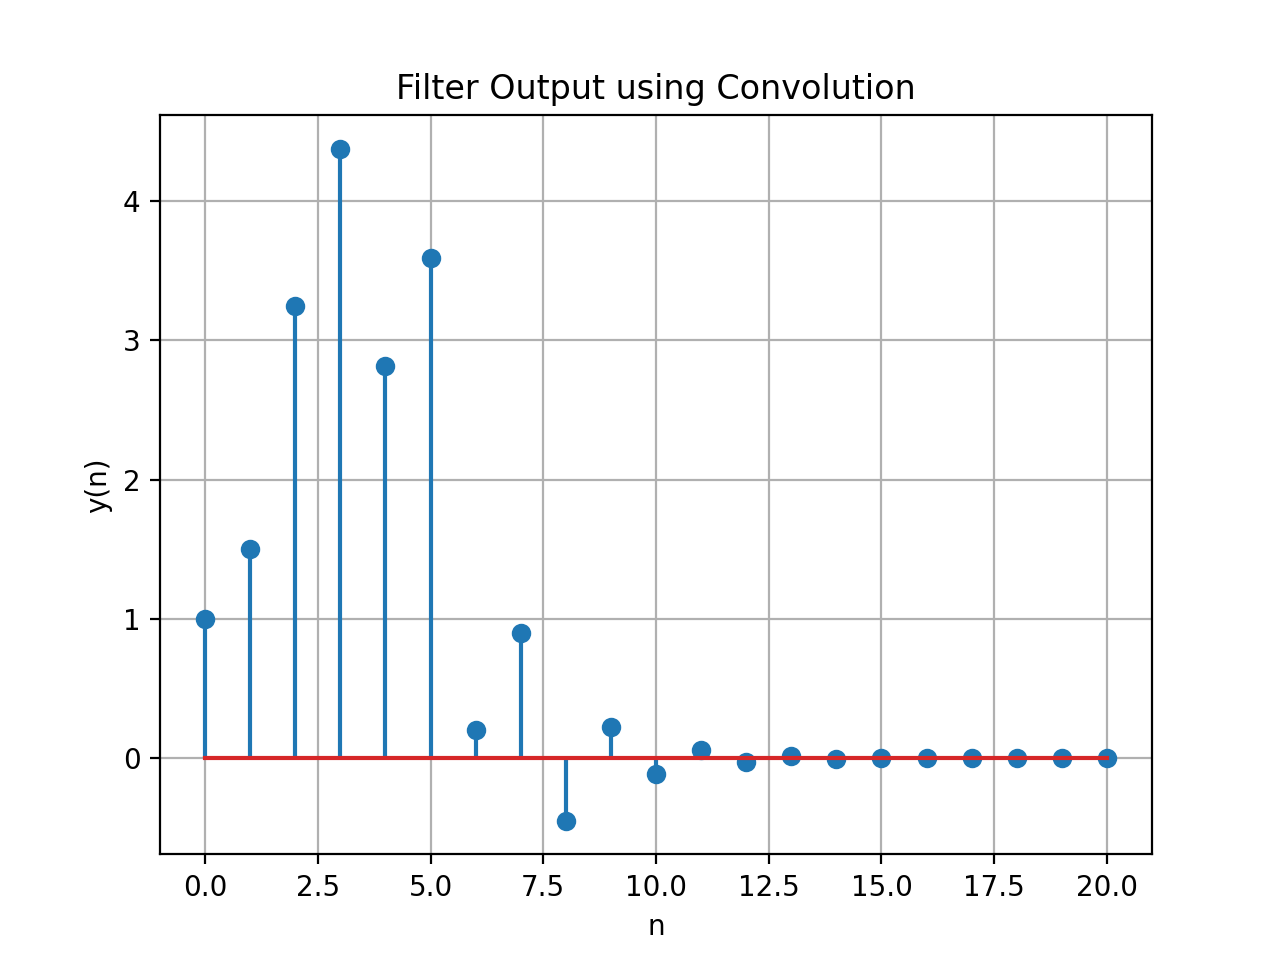
\includegraphics[width = \columnwidth]{figs/ynconv.png}
        \caption{Convolution of $x\brak{n}$ and $h\brak{n}$ using toeplitz matrix}
        \label{5.9}
      \end{figure}
      \begin{lstlisting}
    wget https://github.com/Pradeep8802/EE3900-Digital-Signal-Processing/tree/main/Assignment1/codes/5.9.py
      \end{lstlisting}
    
      From $\eqref{eq:convolution}$,we express $y\brak{n}$ as
      \begin{align}
        y\brak{n} &= \sum_{k = -\infty}^{\infty}x\brak{k}h\brak{n-k}
      \end{align}
      To understand how we can use a Toeplitz matrix, we will see what we are doing in $\eqref{eq:convolution}$ 
      \begin{align}
        y\brak{0} &= x\brak{0}h\brak{0}\\
        y\brak{1} &= x\brak{0}h\brak{1} + x\brak{1}h\brak{0}\\
        y\brak{2} &= x\brak{0}h\brak{2} + x\brak{1}h\brak{1} + x\brak{2}h\brak{0}\\
        . \nonumber&\\ 
        .& \nonumber
      \end{align}
      The same thing can be written as,
      \begin{align}
        y\brak{0} &= \myvec{h\brak{0} & 0 & 0 &.\,&.\,&.0}\myvec{x\brak{0}\\x\brak{1}\\x\brak{2}\\ . \\.\\x\brak{5}}\\
        y\brak{1} &= \myvec{h\brak{1} & h\brak{0} & 0 & 0 &.\,&.\,&.0}\myvec{x\brak{0}\\x\brak{1}\\x\brak{2}\\ . \\.\\x\brak{5}}\\
        y\brak{2} &= \myvec{h\brak{2} & h\brak{1} & h\brak{0} & 0& .\,&.0}\myvec{x\brak{0}\\x\brak{1}\\x\brak{2}\\ . \\.\\x\brak{5}}\\
        . & \nonumber \\
        .& \nonumber
      \end{align}
      Using Toeplitz matrix of $h\brak{n}$ we can simplify it as,
      \begin{align}
        y\brak{n} &= \myvec{h\brak{0} & 0 & 0 &.\,&.\,&.\,0 \\
          h\brak{1} & h\brak{0} & 0 & .\,&.\,&.\,0 \\
          h\brak{2} & h\brak{1} & h\brak{0} & .\,&.\,&.\,0 \\
          &&..\\&&..\\ 0 & 0 &  0 &.\,&.\,&.\, h\brak{m-1}}\myvec{x\brak{0}\\x\brak{1}\\x\brak{2}\\ . \\.\\x\brak{5}}\label{eq:5.9}
      \end{align}
      Now from $\eqref{def:xn}$ we will take n 
      \begin{align}
        x\brak{n} &= \myvec{1\\2\\3\\4\\2\\1}
      \end{align}
      And from $\eqref{eq:h_n_def}$ we will take some values of n,
      \begin{align} 
        h\brak{n} &= \myvec{1 \\ -0.5 \\ 1.25 \\. \\ . }
      \end{align}
      Now using $\eqref{eq:5.9}$,
      \begin{align}
        y\brak{n} &= x\brak{n}*h\brak{n}\\
        &= \myvec{1 & 0 & 0 &.\,&.\,&.\,0 \\
          -0.5 & 1 & 0 & .\,&.\,&.\,0 \\
          1.25 & -0.5 & 1 & .\,&.\,&.\,0 \\
          &&..\\&&..\\ 0 & 0 &  0 &.\,&.\,&.\, }\myvec{x\brak{0}\\x\brak{1}\\x\brak{2}\\ . \\.\\x\brak{5}} \\
        &= \myvec{1\\1.5\\3.25\\.\\.\\.}
        \label{eq:topliz}
      \end{align}
    The above equation \eqref{eq:topliz} is the convolution of $x(n)$ and $h(n)$
      
      
      
    \item Show that
      \begin{equation}
        y(n) =  \sum_{k=-\infty}^{\infty}x(n-k)h(k)
      \end{equation}
    \solution From \eqref{eq:convolution}, 
      \begin{align}
        y(n) = \sum_{k=-\infty}^{\infty}x(k)h(n-k)
      \end{align}
      Replacing $n-k$ with $a$,we get
      \begin{align}
        y(n) &= \sum_{n-a=-\infty}^{\infty}x(n-a)h(a)\\
        &=\sum_{-a=-\infty}^{\infty}x(n-a)h(a)\\
        &=\sum_{a=-\infty}^{\infty}x(n-a)h(a)
      \end{align}
    \end{enumerate}
\section{DFT and FFT}
\begin{enumerate}[label=\thesection.\arabic*]
\item
Compute
\begin{equation}
X(k) \define \sum _{n=0}^{N-1}x(n) e^{-\j2\pi kn/N}, \quad k = 0,1,\dots, N-1
\end{equation}
and $H(k)$ using $h(n)$.
\item Compute 
\begin{equation}
Y(k) = X(k)H(k)
\end{equation}
\item Compute
\begin{equation}
 y\brak{n}={\frac {1}{N}}\sum _{k=0}^{N-1}Y\brak{k}\cdot e^{\j 2\pi kn/N},\quad n = 0,1,\dots, N-1
\end{equation}
\\
\solution The following code plots Fig. \ref{fig:ynconv}. Note that this is the same as 
$y(n)$ in  Fig. 
\ref{fig:xnyn}. 
%
\begin{lstlisting}
wget https://github.com/AvinashNayak27/digital/blob/master/codes/yndft.py
\end{lstlisting}
\begin{figure}[!ht]
\centering
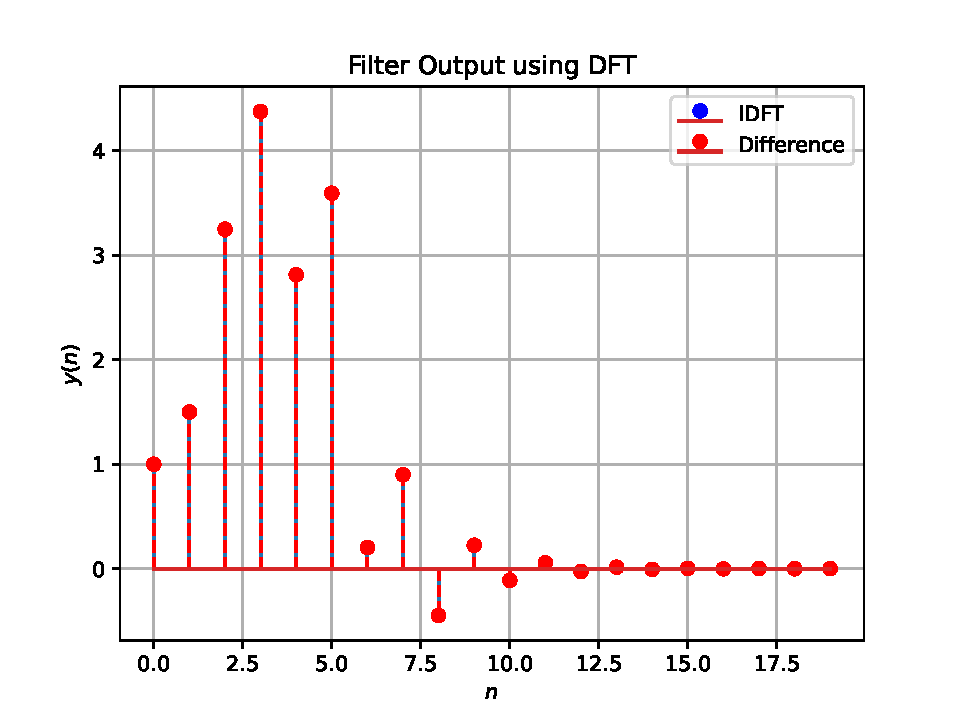
\includegraphics[width=\columnwidth]{./figs/yndft}
\caption{$y(n)$ from the DFT}
\label{fig:yndft}
\end{figure}

\item Repeat the previous exercise by computing $X(k), H(k)$ and $y(n)$ through FFT and 
IFFT.
\item Wherever possible, express all the above equations as matrix equations.
\item Verify the above equations by generating the DFT matrix in python.
\end{enumerate}
%
\section{Exercises}

Answer the following questions by looking at the python code in Problem \ref{prob:output}.
\begin{enumerate}[label=\thesection.\arabic*]
\item
The command
\begin{lstlisting}
	output_signal = signal.lfilter(b, a, input_signal)
	\end{lstlisting}
in Problem \ref{prob:output} is executed through the following difference equation
\begin{equation}
\label{eq:iir_filter_gen}
 \sum _{m=0}^{M}a\brak{m}y\brak{n-m}=\sum _{k=0}^{N}b\brak{k}x\brak{n-k}
\end{equation}
%
where the input signal is $x(n)$ and the output signal is $y(n)$ with initial values all 0. Replace
\textbf{signal.filtfilt} with your own routine and verify.
%
\item Repeat all the exercises in the previous sections for the above $a$ and $b$.

\item What is the sampling frequency of the input signal?
\\
\solution
Sampling frequency(fs)=44.1kHZ.
\item
What is type, order and  cutoff-frequency of the above butterworth filter
\\
\solution
The given butterworth filter is low pass with order=2 and cutoff-frequency=4kHz.
%
\item
Modifying the code with different input parameters and to get the best possible output.
%
\end{enumerate}

\end{document}
